\section{Implementation}
\begin{figure}[H]
    \centering 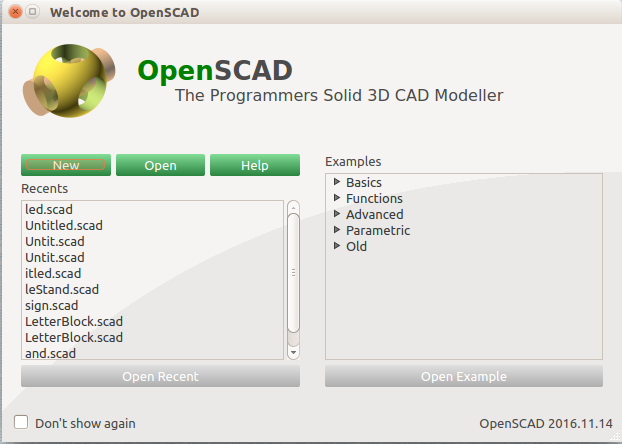
\includegraphics[width=0.7\linewidth]{images/output/1.png}
    \caption{StartUp Screen for OpenSCAD}
    \label{fig:1}
\end{figure}
\subsection{Multithreading}
In order to understand how we have attempted to implement multithreading for geometric rendering we need to understand the problem in substantial detail.\\
Even though it has been mentioned before profoundly, we feel the need the reiteration of what OpenSCAD is and how it achieves its goals. OpenSCAD is a 3D modeler i.e. it creates 3D models. The user interaction is done through a scripting language. This language describes the object(s) that the user wishes to create. This system has been put in place for the following reasons:
\begin{itemize}
	\item The fundamental geometric constructs of general purpose programming languages are too complex for an avergae computer user to learn and master. Even though ultimately, these constructs are being used to make everything in OpenSCAD but it is very difficult to expose the user to such tools. They are a little too fundamental and esoteric for the software to be of any help to your average modeler or designer who are unlikely to have much expertise of computer programming.\\
	That is why it becomes very important that the user is given an interface which has much less steeper learning curve than direct usage of geometric libraries. The OpenSCAD modelling language is just the interface for the job.
	\item Freedom and flexibilty of designing can be greatly compromised if only GUI constructs are used for modelling purpose. It is essential to give the user enough power to create complex and intricate designs easily without havnig to be limited by what the GUI has to offer. The modelling language, while being very intuitive is in fact very powerfull. The learning curve is much more user friendly without compromising the user's ability to make powerful designs. It saves a lot of time to use a higher abstraction of geometric constructs than to use the fundamentals them selves.\\
	The OpenSCAD modelling language thrives for the reasons any high level language thrives over a more machine related language. Time and effort of the programmer is saved and readability, portability are gained.
\end{itemize}
Here is a snapshot of the a model description using the above mentioned langauage:
\begin{figure}[H]
    \centering 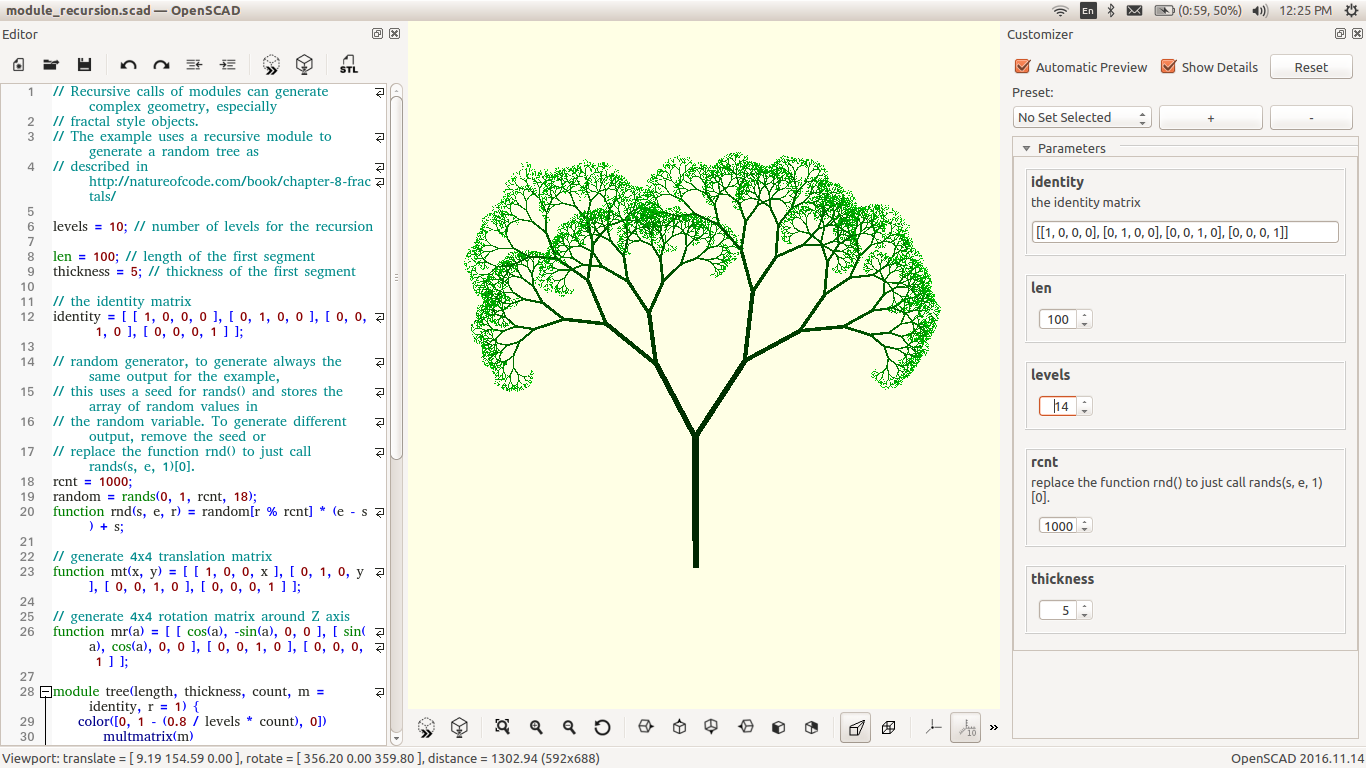
\includegraphics[width=\linewidth]{images/output/5.png}
    \caption{StartUp Screen for OpenSCAD}
    \label{fig:1}
\end{figure}
This language is parsed and converted into an Abstract Syntax Tree. This AST is used to turn descriptions of the objects into their graphic form. The AST is fed to an evaluator which reads the entire abstract syntac tree and turn it into a nodal tree. Each node in the tree represents geometric forms to be drawn. Once the node tree has been generated, references of this are pased around in order to accomplish various things. The same node tree can be used to generate the preview of the model using CSG and the same node tree is used to render the model. All of this can be summarised by the following flow chart:
\begin{figure}[H]
    \centering 
    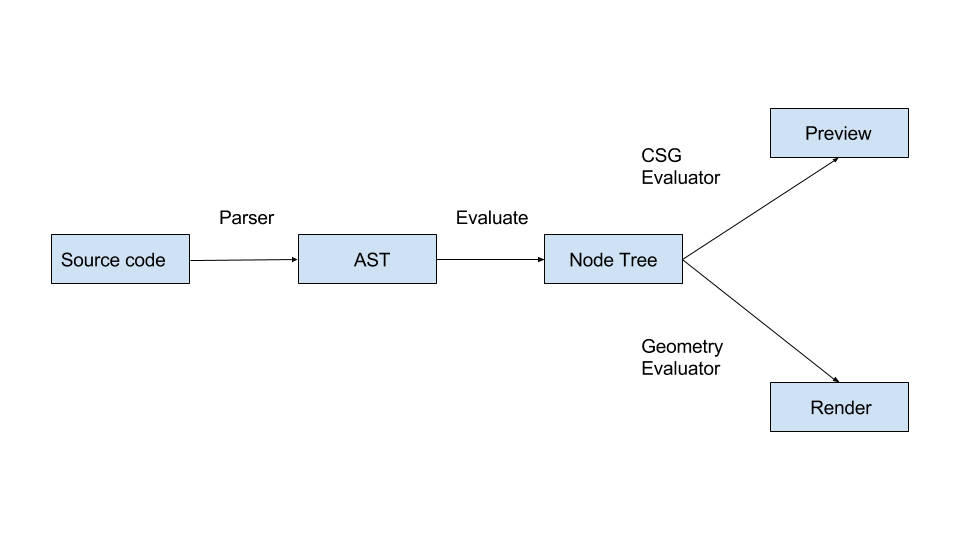
\includegraphics[width=\linewidth]{images/flowchart.png}
    \caption{Working flow of OpenSCAD}
\end{figure}
The first thing that was needed to be done was understanding the flow of the software and figuring out what sections of code needs to be parallelized. After forming a firmer understanding of the problem, it was required to check all the relevant data structures involved in evaluating the tree nodes. It was also be checked if any data structures used were needed to be modified or not. After fixing the appropriate data structures, all the feasible and plausible approaches were to be explored. Each approach has been evaluated on its merits and feasibility. Among all the options the one which is works well across all platform has been chosen. It goes without saying that the chosen solution has to meet all the requirement and implement the solution efficiently. After going through all of this the implementation began. The diagram below depicts the intended approach:
\begin{figure}[H]
    \centering 
    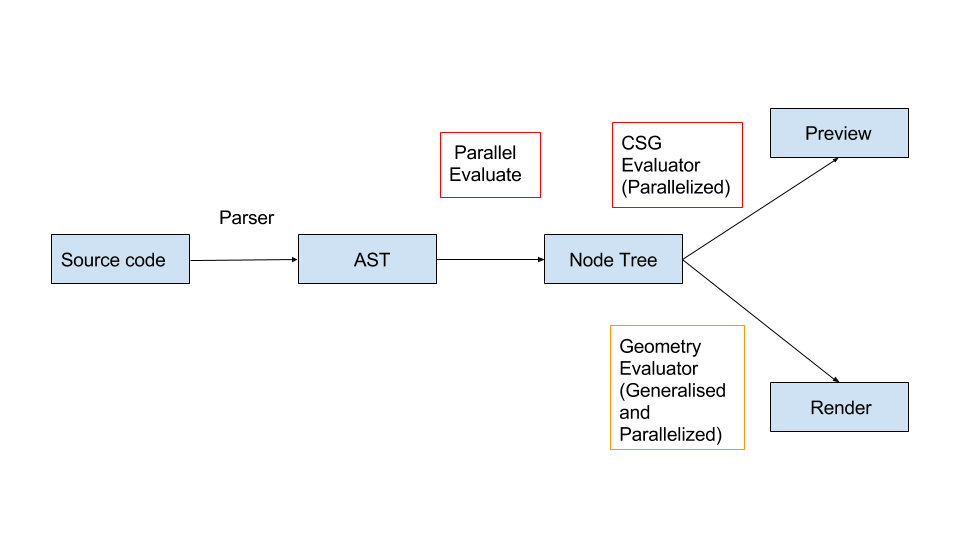
\includegraphics[width=\linewidth]{images/finalflow.png}
    \caption{Flowchart for the solution}
\end{figure}
During the implementation it was important to understand how the code works otherwise it will not have been possible to alter that code or even add to it. As OpenSCAD's GUI opens up, the code in the MainWindow.cc file is run. From here, the user can do many things but for our intent we are only going to focus on what happens when F6 is pressed. F6 is to issue the render command which is carried out via the actionRender() function. Following the flow of code from this function, it was descovered that the node tree is getting traversed recursively using the traverse function defined in the nodeVisitor.cc file. As mentioned, this function traverses each node is the node tree starting from the root node and then visiting each node recursively. Together with visiting each node, this function also calls out the accept() function on each node which is used to process the node further.\\
The whole point of multithreading was to parallelise this process of evaluating nodes. In its fundamental form, this is problem of applying parralelism to tree traversal. This parralelism can be achieved by simplying creating a new thread each time a new branch of the tree is to be traversed. But one may see, that this approach is not thread safe. First of all, the nodes that are getting visited must be accounted for in some sort of collection. And if various threads are going to visit the nodes and then update this collection then it becomes very important to make sure that no two threds are ever in a race, competing to update the collection at the same time. Such safety can be achieved by using lock mechanism.\\
This is not even the major problem, the real issue is in making sure that the global resources used by these functions are not unsafe from race conditions or concurrent access. Dealing with this took great effort and careful programming.
\subsection{Halting Mechanism for Render}
Ones the render process has been started, intentionally or unintentionally, there is nothing that can be done to stop the process without closing openSCAD altogether. The rendering process is not instantaneous making this a certain problem. There has to be method that on the user's command can halt an ongoing render process.\\
It is not just that the rendering process is to be stopped, it is also important to somehow perserve the partial work that has been done the rendering process before being halted by the user. This is achieved by caching the work and keeping the cache accesible across compiles in ordet to save time.\\
On carefull examination of the code, it was found that the cancel button was already part of the GUI. It just wasn't doing much usefull stuff to cancel the process. The cancel button is part of the progress widget GUI. And it is required to do is set a boolean variable to true. The variable name is wasCancelled. There is also function that checks the value of this variable to tell whether the process was cancelled or not i.e. the button was pressed or not. This function name is wasCancelled().\\
It is easy see that most pieces of the puzzle are already there. It is just required to place them properly and make them come together.\\
On some rigorous source browsing and consultation with the OpenSCAD developers, it was found that the assignment to true of the variable wasCancelled actually throws a programmer made exception: ProgressCancelException. Our job was to ensure that proper action is taken when this exception is raised. To do so, we had to tweak the visit() function which is responsible for visiting each node in the tree. This function was not singular. There were any overloaded versions of this depending on the type of node being visited. Hence the same work had to be done for each node.\\
After visiting each node, a made to call to a reporting function was made to happen. This function basically communicates to the progress widget about the number of nodes visited by it. The progress bar ranges from 1 to 1000. But this is not the sole purpose of this function, it also check at the end whether the exception has been raised or not. If it finds the exception is raised, it sets in motion a sequence of function calls that lead to safe halt of the render process. The following figure shows the working of the progress report and the cancel button:
\begin{figure}[H]
	\centering
	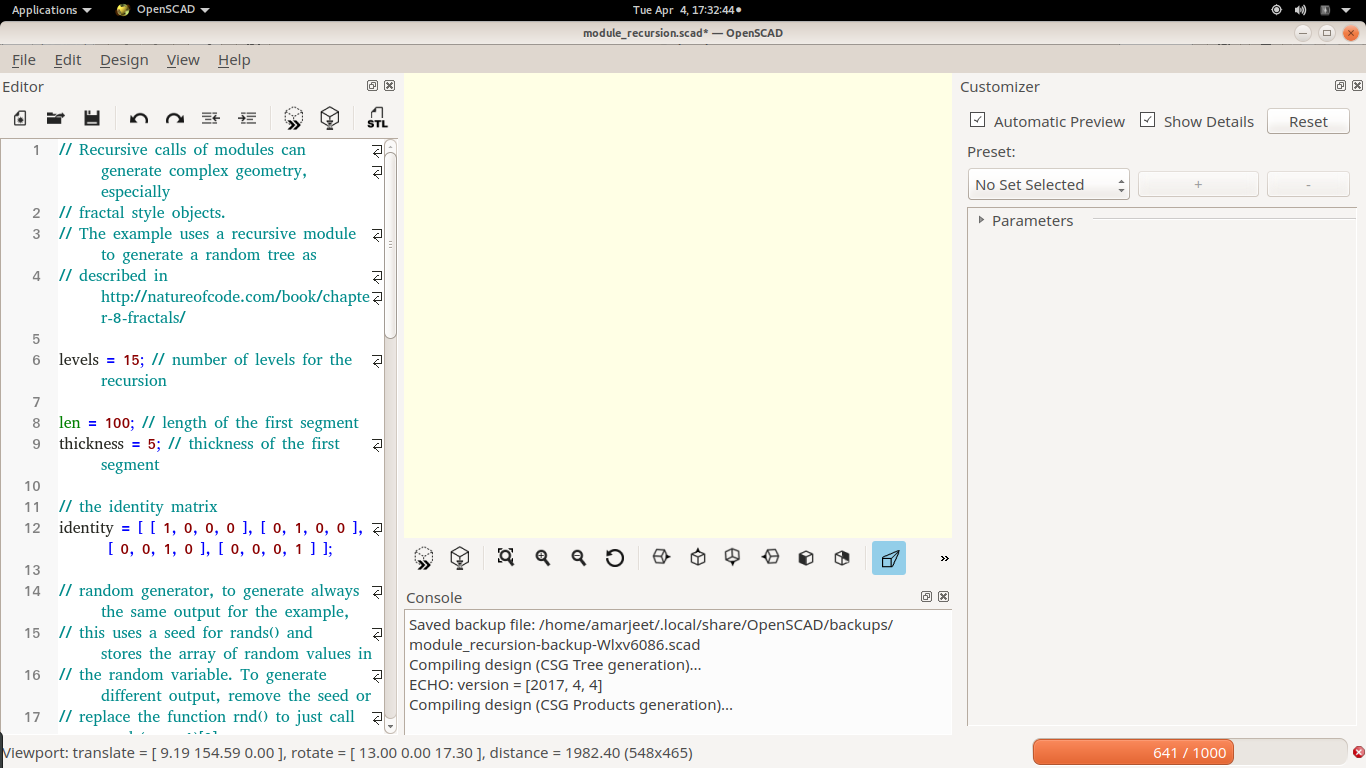
\includegraphics[width=\linewidth]{images/output/progress_widget.png}
	\caption{Progress Widget working}
\end{figure}
\subsection{Finding Root Tag Nodes}
3D models are often formed by taking two separate entities and then merging them using some of the operations like union, intersection and difference. All of this is taken care of at the back end using the node tree. In the node tree, one can have two separate entities as the child of a node and that node being the operation that is to be performed on those entities. As such, in the same model we can have various subsystem of nodes interacting with each other in order to give the final result. This just goes to show that subtrees within the node tree are very much capable of existing independantly. As such, sometimes it is desired by the user to only evaluate a certain branch of subtree of the whole tree. This means everything else in the tree except for that branch is useless for the time being. In order to save time and resources, we have to process and render only that subset.\\
The other parts of the tree are to be ignored. This certainly can not be done by commenting out, or deleting other nodes in the description of the language and then recompiling it. That approach would be very counterproductive.\\
A better way of doing this would be let the whole tree be in place. And when it is time to compile the part of the tree, simply tell the compiler to skip over to the subtree that is required and quit as soon as the compiler is done with that subtree. This way, nothing has to get deleted and only that part is compiled that is actually required. That is why there is a mechanism by which the user is allowed to set for a temporary period of time, a pseudo-root node. This root node can be anywhere in the tree. And when this is to be rendered, the software searches for it in the tree and returns a reference for it.\\
However, since the user is allowed to set multiple pseudo nodes in the tree, the searching function has to store references to all of them. Eventually only the first one of these stored references are used, but others are stored nonetheless. And if infact there are no such pseudo root nodes in the tree, then null is returned, indicating that the actuall root of the tree is to be treated as the root for the next render. It is important that we store all the nodes that have been marked as pseudo-roots. This marking is done by setting an attribute of each node to RootTag. This significanc stems from the fact that it is unnatural and hence useless to have multiple nodes as pseudo roots. For this reason, the user must be reminded as to how many markers have been set. This reminder is given in the form of a warning. In the picture below, one can see how the system worked before:\\
\begin{figure}[H]
	\centering
	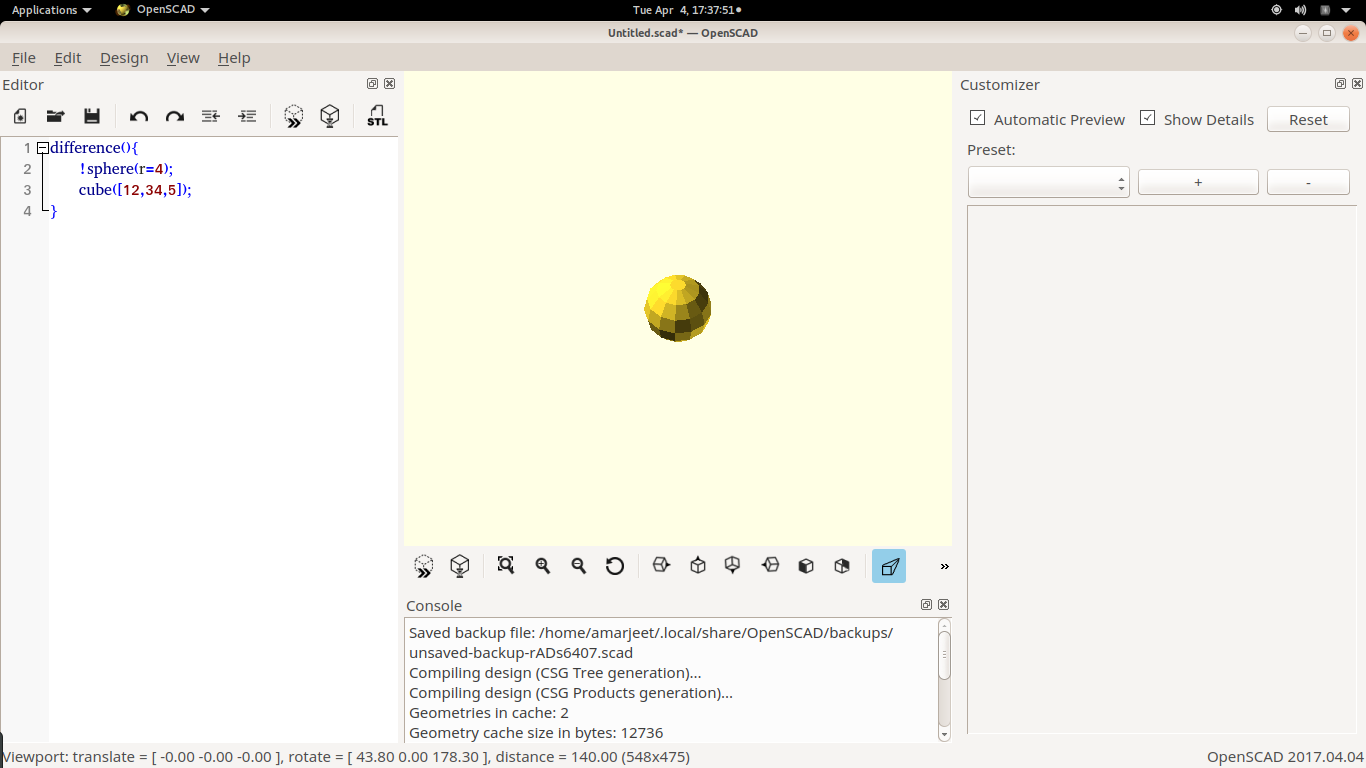
\includegraphics[width=\linewidth]{images/output/before_okay.png}
	\caption{Finding RootTag nodes previously}
\end{figure}
In this figure we can see how only one node has been marked as the pseudo root node (using the exclamation mark). And corresponding to it, we see no warnings because no warnings are due. But consider the following case:\\
\begin{figure}[H]
	\centering
	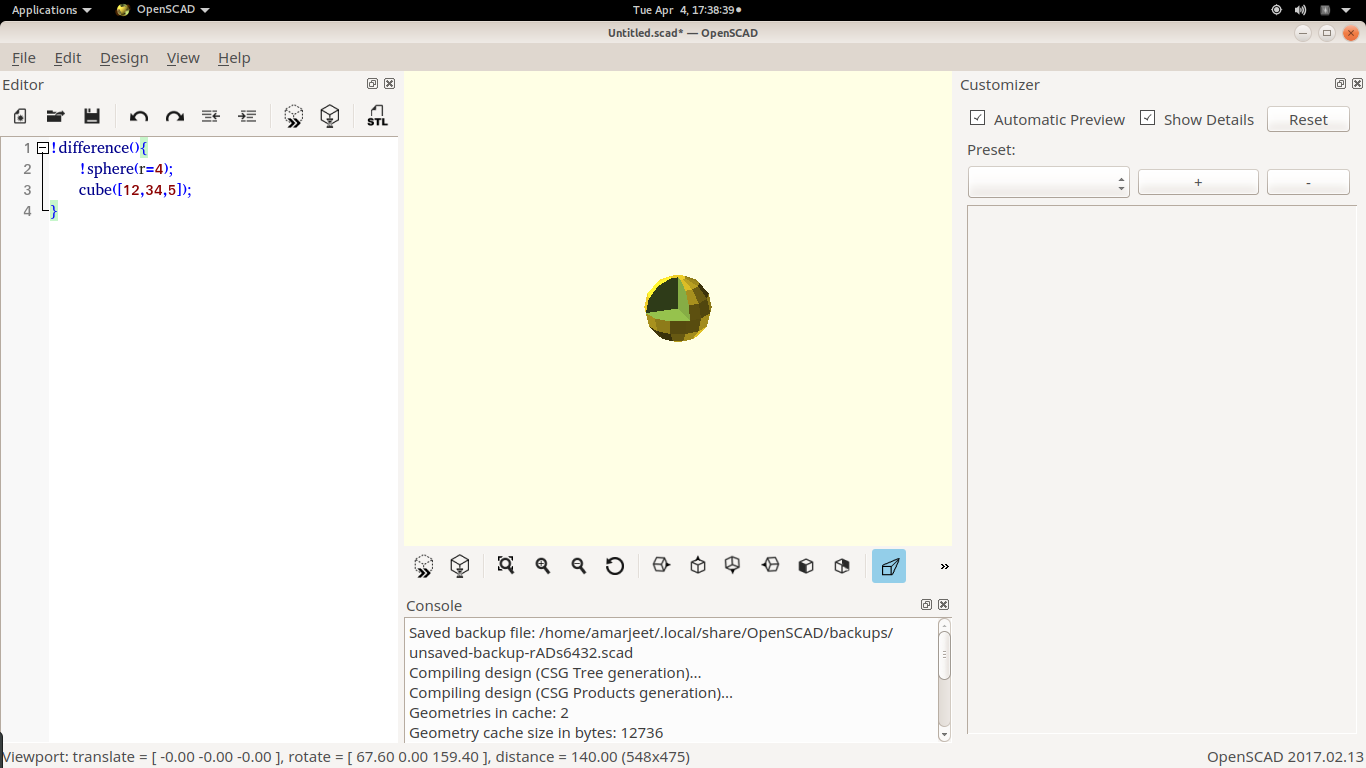
\includegraphics[width=\linewidth]{images/output/before_wrong.png}
	\caption{Finding multiple RootTag nodes previously}
\end{figure}
As seen, even though we had multilpe tags in the model, we didn't get any warnings.
The previous version of this function would search through the tree to find this tag. And the function would return as soon as it has found the first node with this tag or if it has exhausted the search space. In anycase, it was not possible to store all the nodes. We have implemented a solution to this problem by amending this search function.\\
In the present version of this function, we have implemented a lambda function. This lambda function recurses through the entire tree and checks to see if a node is marked or not. All the marked nodes are stored in vector. The result will still be the same as before because only the first element stored in the vector will be rendered, but atleast with this approach, the user is provided with a list of nodes that they have marked unnecessairily. The following figure shows how things are done now:\\
\begin{figure}[H]
	\centering
	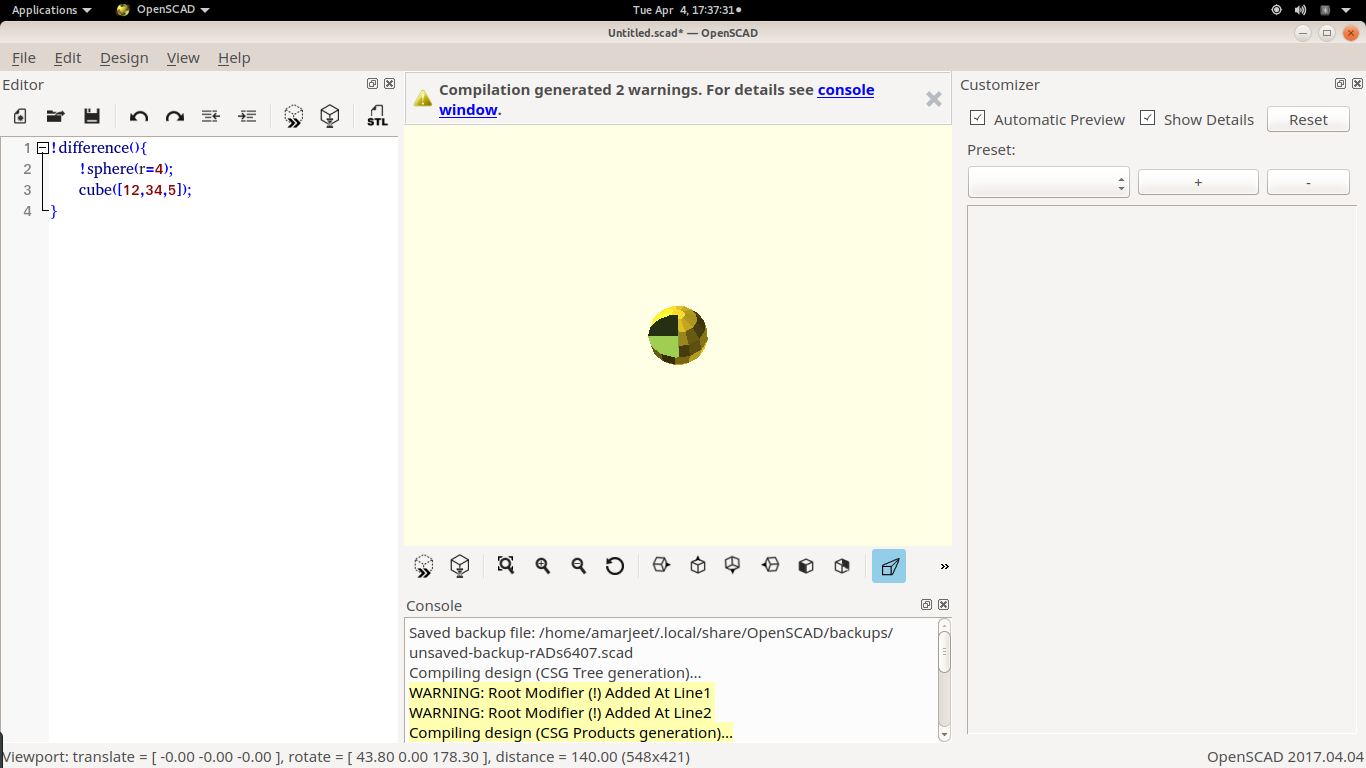
\includegraphics[width=\linewidth]{images/output/now_right.png}
	\caption{Finding multiple RootTag nodes now}
\end{figure}
